\begin{definition}
	Una función $f$ es \textbf{creciente} en un intervalo si para cualesquiera $x_1$ y $x_2$ del intervalo tales que $x_{1} < x_{2}$, se verifica que $f(x_{1}) \leq f(x_{2})$.
\end{definition}
Si la desigualdad es estricta, es decir, si para cualesquiera $x_1$ y $x_2$ tales que $x_1 < x_2$ se verifica que $f(x_{1}) < f(x_{2})$, la función es \textbf{estrictamente creciente}.\\
\newline
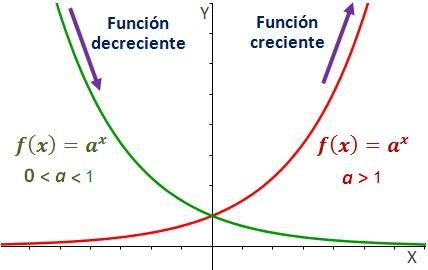
\includegraphics{samples/propiedades/crecienteDecreciente.jpg}\\
\begin{definition}
	Una función $f$ es \textbf{decreciente} en un intervalo si para cualesquiera $x_1$ y $x_2$ del intervalo tales que $x_{1} < x_{2}$, se verifica que $f(x_{1}) \geq f(x_{2})$.	
\end{definition}
Como en el caso anterior, si para cualesquiera $x_1$ y $x_2$ tales que $x_{1} < x_{2}$ se verifica que $f(x_{1}) > f(x_{2})$, la función es \textbf{estrictamente decreciente}.\\
\youtube{cWqJfem3GTk}
\subsubsection{Ejercicios}

\begin{ex}[sol later]
	Determina los intervalos de crecimiento y decrecimiento de la función $f(x)=x^4-2x^2-8$
	\begin{sol}
		\begin{itemize}
			\item Crecimiento: $(-1,0) \bigcup (1,+\infty)$
			\item Decrecimiento: $(-\infty, -1) \bigcup (0,1)$
		\end{itemize}
		\geogebra{rahsjufx}
	\end{sol}
\end{ex}

\vspace{1cm}

\begin{ex}[sol later]
	Determina los intervalos de crecimiento y decrecimiento de la función $f(x)=3x^4-20x^3-6x^2+60x-8$
	\begin{sol}
		\begin{itemize}
			\item Crecimiento: $(-1,1) \bigcup (5, +\infty)$
			\item Decrecimiento: $(-\infty, -1) \bigcup (1,5)$
		\end{itemize}
		\geogebra{z2jageyv}
	\end{sol}
\end{ex}

\vspace{1cm}

\begin{ex}[sol later]
	Determina los intervalos de crecimiento y decrecimiento de la función $f(x)=\dfrac{x+1}{x^2+x-2}$
	\begin{sol}
		\begin{itemize}
			\item Decrecimiento: $\mathbb{R}-\{-2,1\}$ 
		\end{itemize}
		\geogebra{zjmqndnw}
	\end{sol}
\end{ex}

\vspace{1cm}

\begin{ex}[sol later]
	Determina los intervalos de crecimiento y decrecimiento de la función $f(x)=\dfrac{x^4+1}{x^2}$
	\begin{sol}
		\begin{itemize}
			\item Crecimiento: $(-1,0) \bigcup (1, +\infty)$
			\item Decrecimiento: $(-\infty, -1) \bigcup (0,1)$ 
		\end{itemize}
		\geogebra{ct2hh9nx}
	\end{sol}
\end{ex}

\vspace{1cm}

\begin{ex}[sol later]
	Determina los intervalos de crecimiento y decrecimiento de la función $f(x)=\dfrac{x}{1+x^2}$
	\begin{sol}
		\begin{itemize}
			\item Crecimiento: $(-1,1)$
			\item Decrecimiento: $(-\infty, -1) \bigcup (1, +\infty)$ 
		\end{itemize}
		\geogebra{m6jd6rcj}
	\end{sol}
\end{ex}

\vspace{1cm}

\begin{ex}[sol later]
	Trata de observar los intervalos de crecimiento y de crecimiento de las siguientes funciones ayudándote de la representación gráfica de las mismas:
	\begin{itemize}
		\item $f(x) = x + \sqrt{x}$
		\item $f(x) = e^{\dfrac{1}{x}}$
		\item $f(x) = (x-1)e^{-x}$
		\item $f(x) = \dfrac{\ln(x)}{x}$
	\end{itemize}
	\geogebra[stb=true, ai=true]{tc5pbmae}
	\begin{sol}
		Juega con el applet de Geogebra.
	\end{sol}
\end{ex}
